% Diagrama conceptual de la pipeline de O1 (capítulo 3, §3.1).
% Ilustrativo (no es figura de decisión). Compila standalone a PDF y puede
% incluirse en el documento con 
\includegraphics{figuras/o1_pipeline.pdf}.
\documentclass[border=8pt]{standalone}
\usepackage[T1]{fontenc}
\usepackage[utf8]{inputenc}
\usepackage{lmodern}
\usepackage{tikz}
\usepackage{xcolor}
\usetikzlibrary{arrows.meta, positioning, fit, backgrounds, calc}

\definecolor{azul}{HTML}{1F4E79}
\definecolor{azulclaro}{HTML}{DAE8F5}
\definecolor{gris}{HTML}{555555}
\definecolor{verde}{HTML}{2E7D32}
\definecolor{verdeclaro}{HTML}{E4F0E4}

\begin{document}
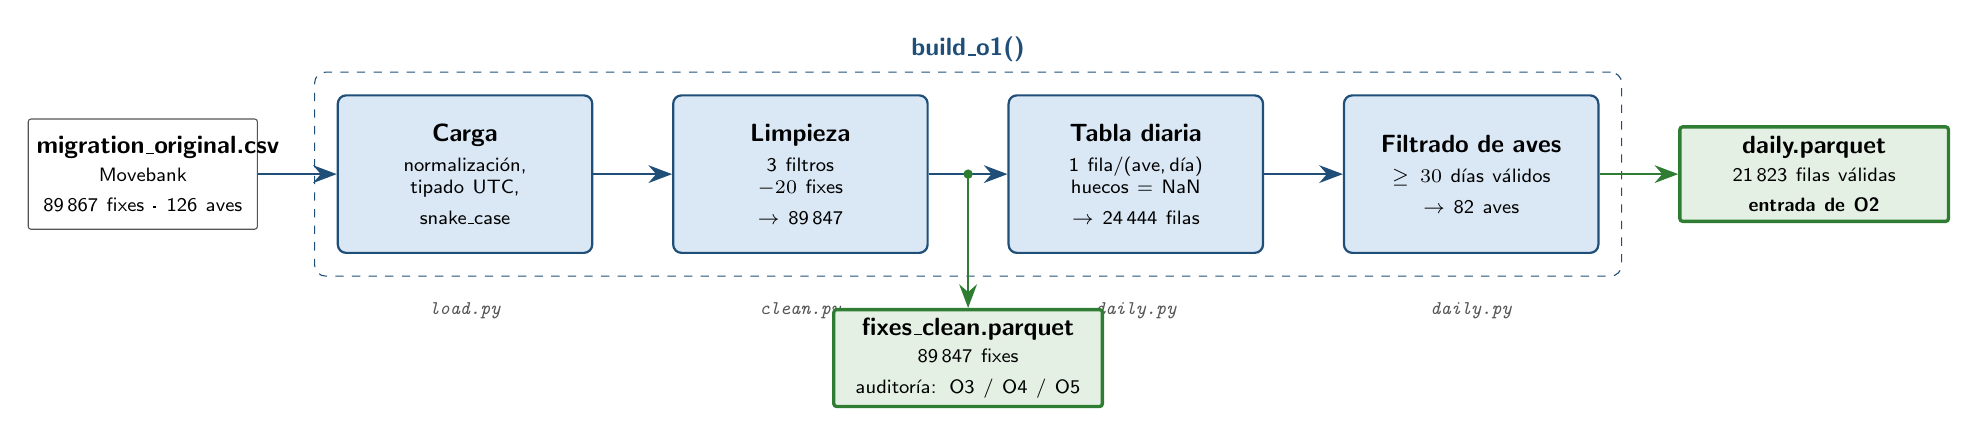
\begin{tikzpicture}[
  font=\sffamily\small,
  stage/.style={rectangle, rounded corners=3pt, draw=azul, thick, fill=azulclaro,
                text width=2.95cm, minimum height=2.0cm, align=center, inner sep=4pt},
  io/.style={rectangle, rounded corners=1pt, draw=gris, fill=white,
             text width=2.7cm, align=center, minimum height=1.4cm, inner sep=3pt},
  salida/.style={rectangle, rounded corners=1pt, draw=verde, very thick, fill=verdeclaro,
              text width=3.2cm, align=center, minimum height=1.2cm, inner sep=3pt},
  arr/.style={-{Stealth[length=3mm]}, thick, azul},
  arrg/.style={-{Stealth[length=3mm]}, thick, verde},
  modlbl/.style={font=\sffamily\scriptsize\itshape, text=gris},
]

% --- Entrada ---
\node[io] (csv) {\textbf{migration\_original.csv}\\[2pt]\scriptsize Movebank\\89\,867 fixes · 126 aves};

% --- Etapas de la pipeline ---
\node[stage, right=1.0cm of csv]  (load)   {\textbf{Carga}\\[3pt]\scriptsize normalización,\\tipado UTC,\\snake\_case};
\node[stage, right=1.0cm of load] (clean)  {\textbf{Limpieza}\\[3pt]\scriptsize 3 filtros\\$-20$ fixes\\$\rightarrow$ 89\,847};
\node[stage, right=1.0cm of clean](daily)  {\textbf{Tabla diaria}\\[3pt]\scriptsize 1 fila/(ave,\,día)\\huecos = NaN\\$\rightarrow$ 24\,444 filas};
\node[stage, right=1.0cm of daily](filter) {\textbf{Filtrado de aves}\\[3pt]\scriptsize $\geq 30$ días válidos\\$\rightarrow$ 82 aves};

% --- Etiquetas de módulo ---
\node[modlbl, below=5mm of load]   {\texttt{load.py}};
\node[modlbl, below=5mm of clean]  {\texttt{clean.py}};
\node[modlbl, below=5mm of daily]  {\texttt{daily.py}};
\node[modlbl, below=5mm of filter] {\texttt{daily.py}};

% --- Flujo principal ---
\draw[arr] (csv)   -- (load);
\draw[arr] (load)  -- (clean);
\draw[arr] (clean) -- (daily);
\draw[arr] (daily) -- (filter);
\coordinate (branch) at ($(clean.east)!0.5!(daily.west)$);

% --- Salidas ---
\node[salida, right=1.0cm of filter] (dailyout)
  {\textbf{daily.parquet}\\[2pt]\scriptsize 21\,823 filas válidas\\\textbf{entrada de O2}};
\node[salida, below=1.7cm of branch] (fixesout)
  {\textbf{fixes\_clean.parquet}\\[2pt]\scriptsize 89\,847 fixes\\auditoría: O3 / O4 / O5};

\draw[arrg] (filter) -- (dailyout);
\fill[verde] (branch) circle (1.7pt);
\draw[arrg] (branch) -- (fixesout.north);

% --- Caja del orquestador ---
\begin{scope}[on background layer]
  \node[draw=azul, dashed, rounded corners=4pt, inner sep=8pt,
        fit=(load)(filter), label={[azul, font=\sffamily\small\bfseries]above:build\_o1()}] {};
\end{scope}

\end{tikzpicture}
\end{document}
